\begin{figure}[t]
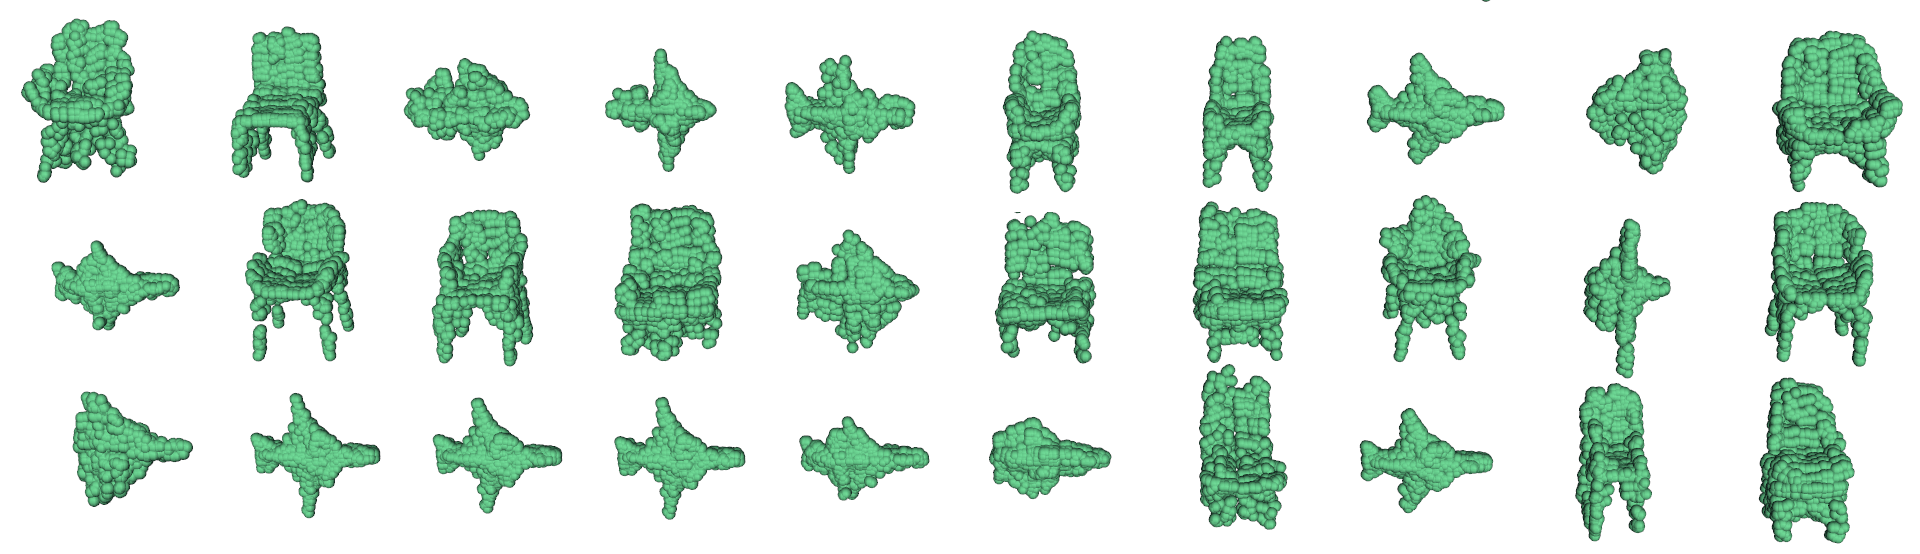
\includegraphics[width=1.0\linewidth]{PCAGAN/images/gallery/chairs_airplane.png}
\vspace{-16pt}
\caption{\small \label{fig:mixed} Results for a mixed category (chair + airplane) showing the ability of our method to capture multi-modal distributions over mixed-category shapes.}
\vspace{-6pt}
\end{figure}

\begin{figure}[t]
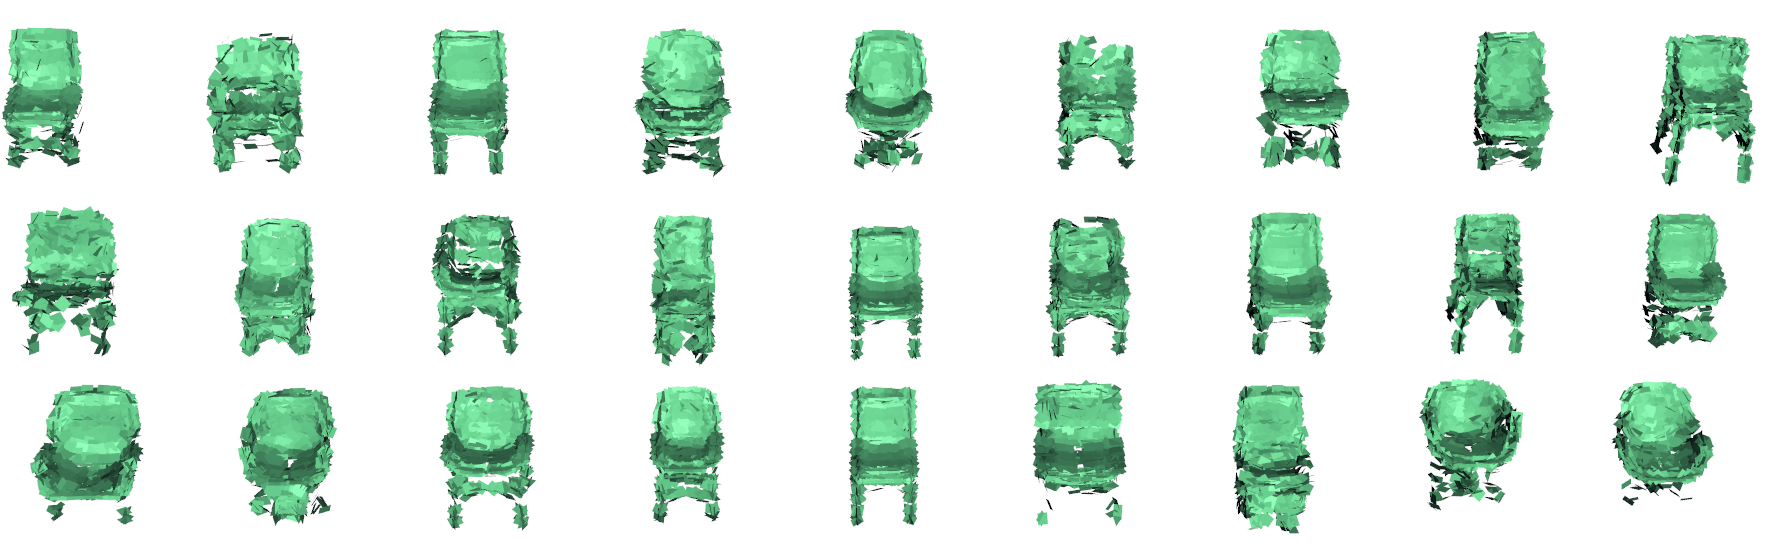
\includegraphics[width=1.0\linewidth]{PCAGAN/images/gallery/chairs_normals.png}
\vspace{-16pt}
\caption{\small \label{fig:normals} Chairs generated with normal. For visualization we shade each point as a square patch centered at the point and oriented by the normal. This shows the ability of our method to generate not only $x,y,z$ coordinates but also incorporate associated point attributes such as normal.}
\vspace{-12pt}
\end{figure}

\section{Experiments}\label{sec:experiments}

\noindent \textbf{Training data.} To generate training data, we use several shape categories from the ShapeNet dataset~\cite{chang2015shapenet}, including chairs, airplanes, cars etc. We sample each shape with 1K Poisson disk sample points using the algorithm described in~\cite{Bowers:2010:PPD}. Poisson disk samples evenly disperse the points over the surface, which turns out to work better at preserving geometric details than using white noise samples. We can easily increase the number of sample points to 4K or 8K and beyond. Unlike voxel-based representations, our method is lightweight, and increasing the sample size only leads to moderate increases in computation resources and time. 

%Those points are sampled in a blue-noise pattern and sorted using the space-partitioning method described in the previous Section.
%Our experiments show that blue-noise sampled points perform slightly better when representing objects with finer geometric details. Each one of the point clouds used in our experiments contain 1024 points.

\vspace{12pt}
\noindent \textbf{Qualitative evaluation.} Figure~\ref{pca:gallery} shows a gallery of results generated using our method for each of the three categories: airplane, chair, and car. The results are generated by randomly sampling the encoding $z$ and demonstrate a variety of shapes within each category. The training is very fast and generally completes within a few minutes. This is an order of magnitude faster than training deep neural networks built upon voxel representations. Figure~\ref{fig:mixed} shows additional results for a mixed category that combines shapes from the chair and airplane datasets. For this mixed category we used $B=300$ basis. The results show the ability of our method to capture the multi-modal distributions over mixed-category shapes.

\vspace{12pt}
\noindent \textbf{Generating multiple point attributes.} Our method can generate points with multiple attributes, such as surface normal, color, by simply appending these attributes to the $(x,y,z)$ coordinates. The overall procedure remains the same except the shape basis is learned over the joint space of positions and normals etc. Figure~\ref{fig:normals} shows chair results generated with normal. The ability to incorporate point attributes is an additional advantage over voxel-based representations (which do not explicitly represent surface information of shapes).

%In the following we present several quantitative and qualitative results to evaluate the our method.
%We start by presenting a quantitative comparison between our model and a competitive PPCA baseline which,
%using the space-partitioning scheme proposed in this paper, yields a similar perceptual quality to 3D-GAN~\cite{wu2016learning}
%as can be observed in Figure~\ref{fig:comparison}.
%We also use this experiment to demonstrate the effect of the number of basis in the generated shapes.
%Second, we present a qualitative evaluation of our technique by using the same training data to query the closest model between
%shapes generated by our method, PPCA and 3D-GAN.
%Third, we show that the GAN learns a manifold of the point clouds by displaying plausible shapes generated while interpolating
%the generator encoding.
%Finally, we demonstrate the ability of our method to generate different types of 3D shapes: chairs, airplanes, cars, tables and
%even multiple categories using same model.
%We also show results where the point clouds are generated with normal annotation.

\begin{table}[t]
\centering
\begin{tabular}{c|ccc|c}
Dataset & GAN(10) & GAN(50) &	GAN(100) &	PPCA (100) \\
\hline
Chairs	& 2.57	& 2.53	& \textbf{2.37}	& 2.88 \\
Airplanes	& 1.96	& \textbf{1.93}	& 1.94	& 2.29 \\
Cars	& 1.45	& \textbf{1.42}	& 1.44	& 1.59 \\
Tables	& 2.88	& 2.68	& \textbf{2.66}	& 3.18 \\
\end{tabular}
\caption{\small \label{tab:quant} Distance (Eq.\ref{eq:chamfer-distance}) between the generated samples and training samples for different generative models. The numbers in parentheses indicate the number of PCA coefficients used for each column. The GAN approach outperforms the PPCA baseline by a considerable margin.}
\vspace{-6pt}
\end{table}

\begin{figure}[t]
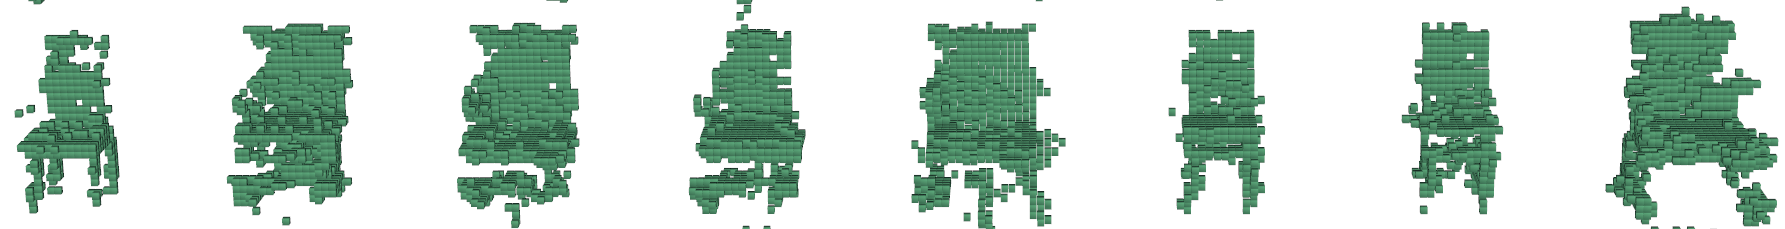
\includegraphics[width=1.0\linewidth]{PCAGAN/images/3DGAN_batch1row.png}
\vspace{-16pt}
\caption{\small \label{fig:3dgan} 3D-GAN result for the chair category. The models are generated by following~\cite{wu2016learning}.}
\vspace{-12pt}
\end{figure}

\begin{figure}[t]
\centering
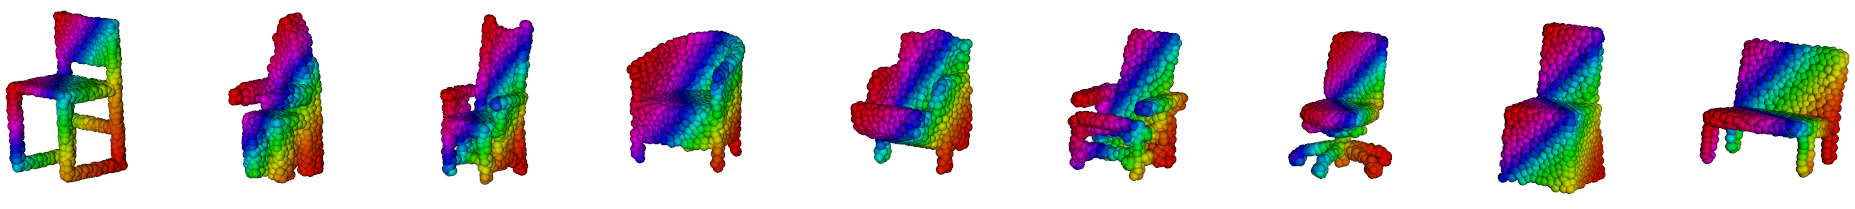
\includegraphics[width=0.8\linewidth]{PCAGAN/images/chairs_xyz_data.png}
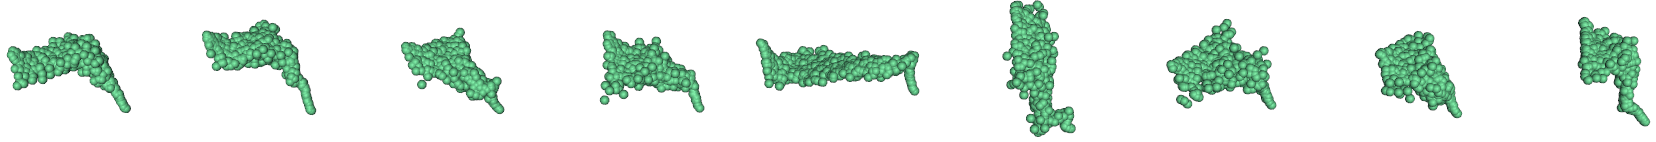
\includegraphics[width=0.8\linewidth]{PCAGAN/images/chairs_xyz_generated.png}
\vspace{-8pt}
\caption{\small \label{fig:chairsxyz} Sorting point clouds using $x+y+z$ values. Top row shows a visualization of the training data using this sorting strategy.
	Bottom row shows the generated shapes for the chair category. They are visually of poor quality compared to kd-tree sorting.}
\vspace{-6pt}	
\end{figure}

\begin{figure}[t]
\centering
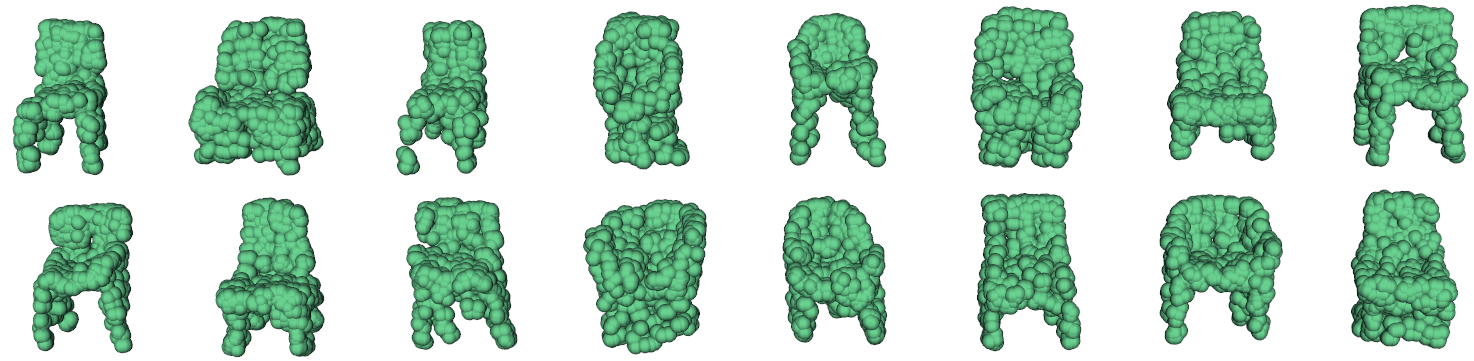
\includegraphics[width=0.8\linewidth]{PCAGAN/images/chairs_1dconv.png}
\caption{\small \label{fig:1dconv} Samples from an alternative GAN architecture using 1D convolutions. Trained using the the point clouds directly.}
\vspace{-12pt}
\end{figure}


\vspace{12pt}
\noindent \textbf{Quantitative evaluation.}
We compare variations of our model to a PPCA baseline~\cite{tipping1999probabilistic}. The PPCA model performs a linear factor analysis of the data using: $y \sim \mathbf{W}x + \mu + \sigma$. The matrix $\mathbf{W}$ is a basis, the latent variables $x \sim N(0, I)$, noise $\sigma \sim N(0, \sigma^2I)$ and the $\mu$ is the data mean. In other words, PPCA learns an independent Gaussian distribution over the coefficients $x$, whereas our approach employs a GAN. We compare PPCA results with variations of our model by changing the number of basis and examining its influence on the quality of the results.
The metric used in the evaluation is defined as follows.
Let $\mathcal{T}$ and $\mathcal{S}$ be the set of training and generated samples, respectively.
We define our distance measure $d(\mathcal{T}, \mathcal{S})$ using a variant of the Chamfer distance, as follows:
\begin{equation}\label{eq:chamfer-distance}
	d(\mathcal{T}, \mathcal{S}) = 
	\frac{1}{|\mathcal{T}|} \sum_{t \in \mathcal{T}} \min_{s \in \mathcal{S}} \norm{t - s}_2 +
	\frac{1}{|\mathcal{S}|} \sum_{s \in \mathcal{S}} \min_{t \in \mathcal{T}} \norm{t - s}_2
\end{equation}
The results can be seen in Table~\ref{tab:quant}. Our approach that uses a GAN to model the distribution of coefficients consistently outperforms the PPCA baseline, which models the distribution as a Gaussian. For the chairs and tables categories the difference between the PPCA and GAN is large, suggesting that the distribution of the coefficients is highly multi-modal. The results by varying the number of bases are also shown in the Table~\ref{tab:quant}. Increasing the number of basis beyond a hundred did not improve our results further.


\vspace{12pt}
\noindent \textbf{Visual comparison to 3D-GAN.} To compare our results with the 3D-GAN model~\cite{wu2016learning}, we followed their description to implement our own version of the algorithm as there is no publicly available implementation that can be trained from scratch. Figure~\ref{fig:3dgan} shows the 3D-GAN results for the chair category. As in~\cite{wu2016learning}, the training data is generated by voxelizing each shape to $64^3$ resolution, and we employ the same hyper-parameters for our GAN model as theirs. Our results, which can be found in Figure~\ref{pca:gallery}, compare favorably to 3D-GAN. In addition, our network is significantly smaller and faster to train.

%shows a set of samples drawn from the generative model for chair category. Visually the results are of better quality than the 3D-GAN and PPCA. However a quantitative comparison with 3D-GAN is difficult since the shape is represented in different ways.


\vspace{12pt}
\noindent \textbf{The role of the \emph{kd-tree}.} The kd-tree induces a shape-dependent but consistent ordering of points across shapes. Moreover the ordering is locality preserving, i.e., two points that are close in the underlying 3D shape are also likely to be close in the list after kd-tree ordering. We believe that this property is critical for the estimating a good basis for the shape representation. In order to verify this hypothesis we consider an alternative scheme where the points are ordered according to their $x+y+z$ value. Although consistent across shapes this ordering does not preserve locality of the points and indeed yields poor results as seen in Figure~\ref{fig:chairsxyz}. However, other data structures that preserve locality such as locality-sensitive hashing~\cite{gionis1999similarity} and random-projection trees~\cite{dasgupta2008random} are possible alternatives to kd-trees.

We also experimented an scheme for generating shapes where \emph{1D~convolutions} on the ordered points are used for both the generative and discriminative models in a GAN framework. Instead of learning a linear shape basis with has wide support over all the points, the 1D-GAN architecture only has local support. Since the ordering is locality sensitive, one might expect that convolutional filters with small support are sufficient for generation and discrimination. This approach can also be robust to a partial reordering of the list due to variations in the shape structures. Moreover, the 1D-GAN can be directly learned on the ordered point list without having to first learn a bases, and is even more compact than the GAN+PCA basis approach. The architecture used for this experiments has the same number of layers with our standard approach. The major difference is in the fact that we use 1D convolutional layers instead of fully connected ones. The generator layers have a filter size of 25 and the first one has 32 filters. The following layers double the number filters of the previous layer. The discriminator is the mirrored version of the generator. Figure~\ref{fig:1dconv} shows the results obtained using the 1D-GAN for the chair category. Remarkably, the generated shapes are plausible, but are ultimately of worse quality than our GAN+PCA approach. Both these experiments suggest that the kd-tree plays a important role for our method.

\vspace{12pt}
\noindent \textbf{Shape interpolation.} Similar to image-based GAN and 3D-GAN, we can perform shape interpolation by linearly interpolating in the encoding space $z$. Specifically, we can pick two encodings $z_1$, $z_2$, linearly interpolate them, and use our generative model to compute the resulting point cloud. The interpolation results are shown in Figure~\ref{pca:interpolation}. As observed, the interpolated shapes are plausible and exhibit non-linearity that cannot be achieved by directly interpolating the shape coefficients.


